\documentclass[addpoints,spanish, 12pt,a4paper,cancelspace]{./include/gexam}

 %%%%%%%%%%%%%%%%%%%%%%%%%%%
 \renewcommand{\documentName} { Sistema de coordenadas cartesianos }
 \renewcommand{\documentContent} { \phantom{ } } 
 \renewcommand{\waterMark} { Modelo 6 } 

 % Configuración del documento.
 \renewcommand{\schoolSubject} { Examen Matemáticas 2º ESO  }
\renewcommand{\school} { IES José de Churriguera  }
\renewcommand{\academicPeriod} { Curso 2022/2023 }

\renewcommand{\autor} { Andrés Giménez Muñoz }
\renewcommand{\emailAuthor} { andresprofemates@outlook.es }
\renewcommand{\autorSing}{ Profesor: Andrés } 
 %%%%%%%%%%%%%%%%%%%%%%%%%%%

\renewcommand\subpartlabel{\thesubpart}
\renewcommand\subpartshook{\renewcommand\makelabel[1]{##1\hfil }} 
 
 %%%%%%%%%%%%%%%%%%%%%%%%%%%
 % Exam configuration
 %\pointsdroppedatright   %% No mostrar la puntuación
 \pointsinrightmargin{} % Para poner las puntuaciones a la derecha. Se puede cambiar. Si se comenta, sale a la izquierda.
 \extrawidth{-1.5cm} %Un poquito más de margen por si ponemos textos largos.
 \marginpointname{ \emph{\points}}
 
 %% Si se comenta no aparecerán los espacios de la solución.
 %\nocancelspace
 
 %% Puntuación a la izquierda.
%  \nopointsinrightmargin 

 %% Esto es de la clase exam. Si dejamos sin comentar \printanswers, se mostraran las soluciones. 
 %% Si la comentamos y dejamos sin comentar \noprintanswers, pues no se muestran las soluciones.
 % \printanswers
 %\noprintanswers
 
 %%%%%%%%%%%%%%%%%%%%%%%%%%%
 
 \begin{document}
 
%  \StudentData{}
%  \GradeTableHeader{}
 
 \justifying

% \begin{center}
%     \fbox{\fbox{\parbox{6.5in}{             
%                 \begin{itemize}
%                     \item Deben aparecer todas las operaciones, no vale solo con indicar el resultado.
%                     \item Se podrán quitar hasta cinco décimas por falta de claridad o rigor en el desarrollo de las respuestas o por una mala presentación.
%                     \item Se valorará que se indiquen las cuentas en línea, realizando las operaciones en el margen.
%                     \item No se puede utilizar la calculadora.
%                 \end{itemize}
%             }}}
% \end{center}
 
 \begin{questions}
    
    %% Gato
    \question Dibuja los puntos en el orden en el que aparece y únelos con segmentos de línea. \\
    \small

    Trazo 1: $(3,4)$ $(6,6)$ $(9,8)$ $(11,9)$ $(12,11)$ $(12,12)$ $(11,13)$ $(10,14)$ $(8,15)$ $(6,15)$ $(4,16)$ $(0,17)$ $(-4,16)$ $(-6,15)$ $(-8,15)$ $(-10,14)$ $(-11,13)$ $(-12,12)$ 
    $(-12,11)$ $(-11,9)$ $(-9,8)$ $(-6,6)$ $(-3,4)$ $(3,4)$ $(2,6)$ $(7,9)$ $(9,11)$ $(9,13)$ $(6,15)$ $(4,16)$ $(0,17)$ $(-4,16)$ $(-6,15)$ $(-9,13)$ $(-9,11)$ $(-7,9)$ $(-2,6)$ $(-3,4)$
    
    Trazo 2: $(2,2)$ $(6,4)$ $(8,4)$ $(8,3)$ $(7,3)$ $(7,2)$ $(5,1)$ $(2,1)$ $(2,2)$ $(-2,2)$ $(-6,4)$ $(-8,4)$ $(-8,3)$ $(-7,3)$ $(-7,2)$ $(-5,1)$ $(-2,1)$ $(-2,2)$
    
    Trazo 3: $(-14,-18)$ $(-16,-15)$ $(-18,-9)$ $(-17,-6)$ $(-18,-6)$ $(-17,-4)$ $(-17,1)$ $(-16,5)$ $(-14,9)$ $(-12,12)$ $(-12,11)$ $(-11,2)$ $(-4,-2)$ $(-4,-6)$ $(-9,-1)$ $(-10,1)$ $(-11,2)$
    $(-10,-3)$ $(-9,-4)$ $(-8,-5)$ $(-3,-9)$ $(3,-9)$ $(8,-5)$ $(9,-4)$ $(10,-3)$ $(11,2)$ $(10,1)$ $(9,-1)$ $(4,-6)$ $(4,-2)$ $(11,2)$ $(12,11)$ $(12,12)$ $(14,9)$ $(16,5)$ $(17,1)$ $(17,-4)$ $(18,-6)$ 
    $(17,-6)$ $(18,-9)$ $(16,-15)$ $(14,-18)$
    
    Trazo 4: $(-10,-3)$ $(-7,-4)$ $(-6,-5)$ $(-5,-6)$ $(-3,-8)$ $(-3,-9)$ $(-2,-9)$ $(-1,1)$ $(1,1)$ $(2,-9)$ $(3,-9)$ $(3,-8)$ $(5,-6)$ $(6,-5)$ $(7,-4)$ $(10,-3)$
    
    Trazo 5: $(-11,3)$ $(-13,1)$ $(-14,-2)$ $(-14,-6)$ $(-13,-10)$ $(-12,-14)$ $(-11,-18)$
    
    Trazo 6: $(12,8)$ $(13,6)$ $(14,3)$ $(15,-1)$ $(15,-4)$ $(16,-7)$ $(16,-10)$ $(15,-13)$ $(14,-16)$ $(13,-17)$
    
    Trazo 7: $(-12,8)$ $(-13,6)$ $(-14,3)$ $(-15,-1)$ $(-15,-4)$ $(-16,-7)$ $(-16,-10)$ $(-15,-13)$ $(-14,-16)$ $(-13,-17)$
    
    Trazo 8: $(11,3)$ $(13,1)$ $(14,-2)$ $(14,-6)$ $(13,-10)$ $(12,-14)$ $(11,-18)$

    \normalsize

    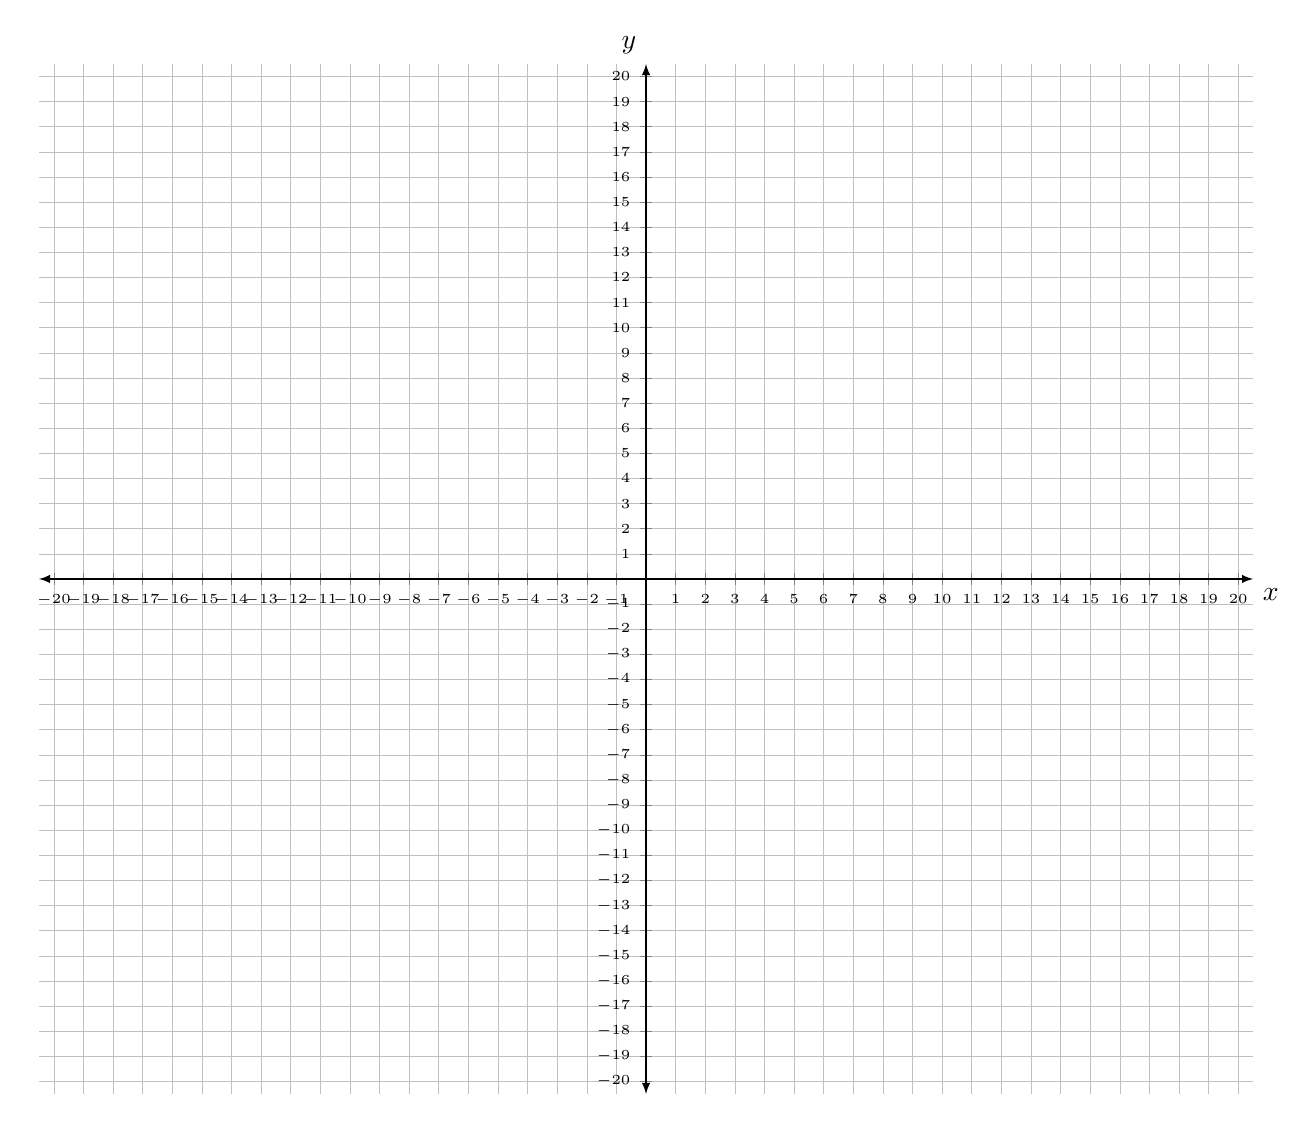
\begin{tikzpicture}[scale=1]
        \begin{axis}[
            axis x line=center,
            axis y line=center,
            xlabel = {$x$},
            ylabel = {$y$},
            xmin=-20,xmax=20,
            ymin=-20,ymax=20,
            xtick distance=1, 
            ytick distance=1, 
            grid=both,
            grid style={line width=.1pt, draw=gray!10},
            major grid style={line width=.2pt,draw=gray!50},
            axis lines=middle,
            axis line style={<->},
            minor tick num=0,
            enlargelimits={abs=0.5},
            axis line style={latex-latex},
            ticklabel style={font=\tiny},
            % ticklabel style={font=\tiny,fill=white},
            % xlabel style={at={(ticklabel* cs:1)},anchor=north west},
            % ylabel style={at={(ticklabel* cs:1)},anchor=south west},
            xlabel style={below right},
            ylabel style={above left},
            width=17cm,
        ]
        
        \end{axis}

    \end{tikzpicture}

\end{questions}
 
\end{document}